\documentclass[10pt,twocolumn,letterpaper]{article}
\usepackage[margin=0.73in,columnsep=0.25in]{geometry}
\usepackage[T1]{fontenc}
\usepackage{mathptmx}
\usepackage{amsmath,amssymb,graphicx,booktabs,tabularx,array,microtype}
\usepackage[font=small,labelfont=bf]{caption}
\usepackage{xcolor}
\usepackage[breaklinks=true,colorlinks=true,linkcolor=blue!45!black,citecolor=blue!45!black,urlcolor=blue!45!black]{hyperref}
\usepackage{enumitem}
\usepackage{placeins}
\setlength{\parindent}{1em}
\setlength{\parskip}{0pt}
\raggedbottom
\setlength{\textfloatsep}{10pt plus 2pt minus 2pt}
\setlength{\floatsep}{8pt plus 2pt minus 2pt}
\setlength{\intextsep}{10pt plus 2pt minus 2pt}
\setlist{nosep,leftmargin=*}
\renewcommand{\topfraction}{0.94}
\renewcommand{\bottomfraction}{0.85}
\renewcommand{\textfraction}{0.06}
\renewcommand{\floatpagefraction}{0.82}
\newcommand{\R}{\mathbb{R}}
\newcommand{\concat}{\operatorname{CONCAT}}
\newcommand{\softmax}{\operatorname{softmax}}
\newcommand{\sigmoid}{\operatorname{sigmoid}}
\newcommand{\pathcode}[1]{\texttt{\detokenize{#1}}}
\graphicspath{{figures/}}

\hypersetup{pdftitle={GNN-Based BERT for Understanding Context from Music},pdfauthor={MD Ashraful Haque Bhuiyan and Wasif Mahtab Hannan},pdfsubject={CSE425 Neural Networks final project report}}

\title{\LARGE\bfseries GNN-Based BERT for Understanding Context from Music}
\author{MD Ashraful Haque Bhuiyan --- Student ID: 22301304\\
Wasif Mahtab Hannan --- Student ID: 23301705\\
BRAC University\\
CSE425 --- Neural Networks}
\date{}

\begin{document}
\twocolumn[\maketitle
\begin{center}\begin{minipage}{0.94\textwidth}
\begin{abstract}
Music context embraces the acoustic events, instrumentation, timbre, temporal relations, and semantic descriptions. This is a feature of a recording that is linked to it. This project explored the possibility of using graph representations of audio segments to augment. Pre-trained language representations for music-context prediction and retrieval. We developed a reproducible pipeline. For a subset of the Google MusicCaps that were acquired locally (761 records), 760 were usable. After filtering by label, 124 proxy labels with the AudioSet label style were left. DistilBERT encoded natural-language captions, and VQ-VAE encoded the image. DistilBERT encoded natural-language captions, and VQ-VAE encoded the image. GraphSAGE aggregated MFCC/chroma segment features across temporal/acoustic-similarity edges. We evaluated a A graph classifier, one based on a mel-spectrogram CNN, and four variants of multimodal classification are evaluated. The following classifiers are evaluated: a direct linear text classifier, a graph classifier against a mel-spectrogram CNN, and four variants of multimodal classification. A dual encoder for graph caption that relies on contrastive learning. GraphSAGE's test Macro-/Micro-F1 scores were 0.1006/0.2936, which surpassed the CNN's 0.0873/0.2033. The early concatenation had the best macro-F1 score when the ablation budget was equal among all 4 epochs. 0.1770, with Micro-F1 of 0.3361; cross-attention reached 0.0685/0.2628. The newly trained 8-epoch DistilBERT. The highest observed micro-F1 was 0.3392 from the baseline. Video-to-caption translation in all languages. Audio-to-captions and video-to-captions translation in all languages by Symmetric InfoNCE training. caption-to-audio R@10 of 0.3772 and 0.3860, respectively. These results suggest that structural audio is worthy of further study. Limited-supervised representations and simple multimodal fusion. The results are limited due to small and unbalanced sample sizes. Below, the data set is split in half, and a different random seed and unequal budget are used.
\end{abstract}
\end{minipage}\end{center}\vspace{0.6em}]

\section{Introduction}
Music-context understanding involves more than identifying isolated acoustic patterns. A microphone or similar audio source and the type of sound generated by the instrument. expressed relates to repetition and relationships between. Musical segments rely on the structure of time. Captions Add another source of information---a human description may Specify instruments and/or production qualities, The attributes of style that must be derived from sound. Such complementary views are used to motivate models that combine Natural-language semantics for acoustic representations. Convolutional and recurrent models are helpful for identifying and abstracting acoustics patterns [1]. However, the sequence and spectrogram representations that they commonly use Set up an explicit separate relation between acoustically similar but nonadjacent segments. The introduction of a graph is given by the points below: such connections directly. Concurrently, pre-trained language encoders can be used to project captions into the space of contextually encoded token representations. The main issue is whether such representations can be effectively fused when used in conjunction with training data. are limited. To answer this question, we analyzed a subset of audio clips and captions from Google MusicCaps that we acquired locally [2, 10]. The project title is in reference to the BERT family of language models used, and the particular checkpoint evaluated was indeed distilbert-base-uncased. The task was set to be prediction. Uses AudioSet-like metadata labels that are retained as proxy information for music context. Not all contextual dimensions were assessed. Mentioned in the motivation, extracted lyrics, or inferences of human Developed from an annotated emotion data set. The following four research questions were followed in the experiments. RQ1: How Can captions by themselves be used for multi-label context prediction? RQ2: Is the performance of graph-based audio modeling better than a mel-spectrogram CNN when the split and training budget are the same? RQ3: What strategy of fusion is the best when paired data is limited, compared to uni-modal variants? RQ4: Can a graph encoder and a caption encoder learn a useful common retrieval What would be the benefits of using contrastive training for space? The contributions include a reproducible pipeline for the preparation of audio-caption graphs and a segment graph based on MFCC/chroma. Included are features and temporal/similarity relations; a matched-budget A four-way fusion ablation; A bi-directional contrastive retrieval experiment. Saved configurations, vocabularies, learning histories, checkpoints, For its attention outputs and for its tests, it reports the following comparisons: traceable. The classification and summary of the separate classification are presented in Figure 1. retrieval paths.

\begin{figure*}[t]
\centering
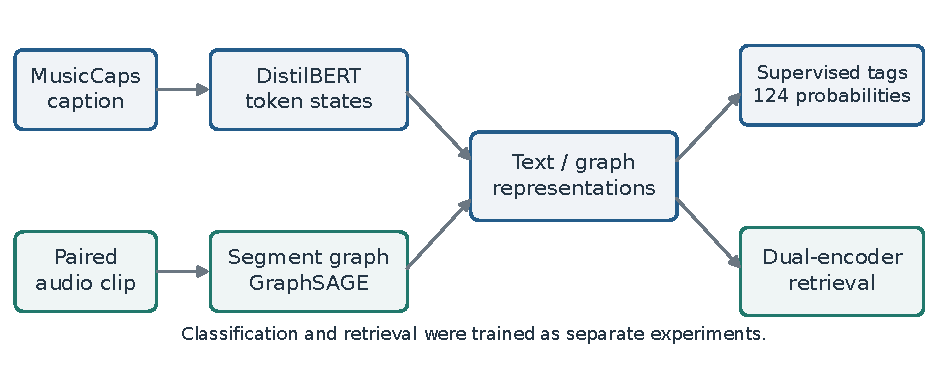
\includegraphics[width=0.92\linewidth]{fig1_system.pdf}
\caption{Overall system schematic. Caption and graph encoders support supervised tag prediction and a separately trained contrastive retrieval model. The diagram depicts implemented data flow, not a jointly trained four-task network.}
\label{fig:system}
\end{figure*}

\section{Related Work}
\textbf{Language representations.} Language representations. BERT introduced bidirectional Using task-specific output layers for pretraining and adaptation of transformers [3]. DistilBERT distills language-model knowledge into a smaller encoder [4]. Its first-token representation (FT) was used in a context-specific manner for classification. and retrieval, and its full token sequence for cross-attention. The comparisons between different language-model checkpoints are not possible. was performed.

\textbf{Representations of music on graphs.} Representations of music on graphs. GraphSAGE learns Node features are aggregated in neighborhood aggregation functions [5]. Its mean aggregator is appropriate for our little graphs. Nodes represent audio segments, and edges represent explicit relationships. Graph attention networks learn attention rather than graph. They offer a potential solution to the problem of weights over graph neighborhoods [6]. However, these were not assessed here, as they are part of the extension. In music information Retrieval, convolutional, and recurrent networks have been developed. He has studied methods for audio feature extraction and temporal summarization [1]. Our mel-CNN is used as a project baseline instead. More than just the paper's structure or conclusions.

\textbf{Contrastive learning and audio--text.} Contrastive learning and audio-text. MusicCaps supplies A set of expert-written descriptions, along with music clips, was released with MusicLM [2]. The CLAP is an example of the broader . . . . A method for synchronizing the language and sound of two encoders. In contrastive objectives [7], a contrastive analysis is employed. A matching representation is distinguished from other competing representations by InfoNCE, which is built on the principle of contrastive predictive coding [8]. We used a symmetric paired-batch variant to graph and caption embeddings. These works inspire the formulation of the numbers; their benchmark numbers are There are no comparable results from not using our data, encoders, and the results of the experiments. Evaluation protocols differ.

\section{Problem Formulation}
A clip is a representation of
\begin{equation}
T_i=(X_i^{\mathrm{audio}},X_i^{\mathrm{text}},G_i,y_i),
\end{equation}
where Xi audio is an audio-derived representation, Xi text is the caption, Gi = (Vi , Ei) is its segment graph, and yi $\in$ \{0,1\} C is a multi-hot context vector with C = 124. The graph is Not separately annotated in the audio file; constructed from the audio. modality. A classifier gives outputs of logits $\ell$ic and probabilities pic = For each label, sigmoid($\ell$ic) independently. Supervised training is performed with positive-weighted binary cross-entropy for a mini-batch of size B:
\begin{equation}
\begin{aligned}
\mathcal{L}_{\mathrm{tags}}=-\frac{1}{BC}\sum_{i=1}^{B}\sum_{c=1}^{C}
\big[&w_c y_{ic}\log p_{ic}\\
&+(1-y_{ic})\log(1-p_{ic})\big].
\end{aligned}
\label{eq:bce}
\end{equation}
Evaluates this expression at the following points: BCEWithLogitsLoss for numerical stability. Weights are were calculated from class frequencies of the training set and they increase Positive contribution of underrepresented classes. The fixed threshold y\textasciicircum{}ic = $\mathbb{1}$[pic $\geq$ 0.5] is used for predictions. A A sigmoid formulation allows for co-occurring tags, and it does not impose mutual exclusivity. Graph representation learning maps Gi to a vector gi . Fusion Combines this with representations of text prior to supervised prediction. For the separate retrieval task, graph and interpret the results. A pair of inputs is grouped into a common metric space by the use of a caption encoder. The ranking goal is to achieve the exact match of the audio-caption, rather than classification of the 124 tags.

\section{Dataset and Preprocessing}
\subsection{Dataset source and local acquisition}
MusicCaps is released by Google in conjunction with the release of MusicLM and includes 5,521 examples of music that are 10 seconds long from AudioSet. along with an aspect list in English and a free text caption written by musicians [2, 10]. These are the public metadata used for this. The project has been pulled from the Google MusicCaps repository. on Hugging Face. It has musiccaps-public.csv records with fields. The boundaries of the excerpt within the YouTube video (YouTube ID + start and end positions of the excerpt) The following are new AudioSet positive labels: start\_s, end\_s, and AudioSet aspect\_list. and caption. Google stands out as the official dataset card. The homepage of the dataset is the MusicCaps page on Kaggle [10]. The public CSV does not offer identifiers or timestamps, but only better than embedding the audio waveform in each row. Following the project acquisition notebook, the corresponding ten-second excerpts were obtained from the referenced YouTube videos and saved as WAV files. The project table, musiccaps\_with\_audio\_paths.csv, shows the original metadata along with a local audio path. and download\_status. The experiments are carried out locally with the usage of the 761. Did not take possession of rows available to the project; they do not "own" them. Include all 5521 entries in the complete MusicCaps release.

\subsection{Audit and target definition}
The total number of records in the locally acquired corpus was 761 (in CSV format). 761 one-to-one correspondence WAV files. The All audio files were found, and no duplicate IDs or null essential files were found. The WAV headers were all readable, and all of the recordings were done in WAV format. The audio took about 1.33 GiB and was in 16-bit PCM format. The statistics of the dataset are shown in Table 1. The average length of the clips was around 10 seconds. Three shorter ones found: 05JAmKFVy44 (9.741 s), 0soVCtJgDTk (9.822 s), and -SWaCArvQug (9.914 s). A consistent duration was achieved by deterministic padding/cropping. after loading. The initial metadata paths were towards Colab's. All of the following were rewritten to valid local paths: environment The raw metadata had 229 AudioSet labels: a long-tailed distribution. MusicCaps aspect fields were found to be too sparse to be used for defining the primary supervised vocabulary. We thus used positive labels in the local metadata as context proxies using the AudioSet style. They are not to be translated. as an all-inclusive taxonomy for genre, mood, musical form, emotion.

\begin{table}[t]
\centering\small
\caption{Dataset audit and prepared split. The experiment used the locally acquired subset, not the full 5,521-example MusicCaps release.}
\label{tab:data}
\begin{tabularx}{\linewidth}{@{}Xr@{}}
\toprule
Property & Value\\
\midrule
CSV records / WAV files & 761 / 761\\
Audio storage & $\approx$1.33 GiB\\
48 kHz, stereo & 571\\
44.1 kHz, stereo & 185\\
44.1 kHz, mono & 5\\
PCM bit depth & 16\\
Raw / retained labels & 229 / 124\\
Minimum tag frequency & 5\\
Usable examples & 760\\
Train / validation / test & 532 / 114 / 114\\
Random seed & 42\\
\bottomrule
\end{tabularx}
\end{table}

\subsection{Vocabulary and split preparation}
The pipeline extracted metadata information from the clips, performed counting on the tag occurrence level, and eliminated the tags that appeared less than five times in an individual clip. Transformed the embedded tags to multi-hot vectors. One example None of the labels survived filtering, so they were removed. This Created 760 examples and 124 labels. Filtering reduced the Most severe lack of supervision, but did not balance the remaining vocabulary or make reliable estimates about less frequent labels. A deterministic iterative multi-label splitter assigned 532 114 examples for training, 114 for validation, and 114 for testing. It assigned examples based on the remaining label needed Split capacity instead of a single row as a single class. instance. This method allows the preservation of uncommon and is suitable for continuous coverage. labels that might be missed by a random division. All retained labels Realized splits appeared in all three splits, and there were disjoint clip IDs. It is a difference between the observed coverage and the actual coverage, the latter of which is a property of the split that is saved, not a universal guarantee of iterative stratification. The corpus-based counts were used for the selection of the vocabulary for the labels. before splitting. Therefore, the reported task is qualified. on this fixed subset and on this fixed label universe. Positive-class Following training weights and model fitting, calibration was performed using training. Calibration was then made based on training. In the former, the examples were selected, and in the latter, the validation measures were used to select the checkpoints. An experiment that was not conducted was a fully training-only vocabulary protocol.

\subsection{Audio preparation}
Waveforms were processed to mono, resampled, and cropped. or stretched out to a set time length. The frame-level MFCC and Chroma features are extracted. These features were divided into 20 temporal segments and then summarized as per feature mean and standard deviation to create a 20$\times$64 node matrix. Similarity construction was based on normalized feature vectors, and the graph encoder used feature Normalization in the forward pass. To prevent re-rendering of features, graph and mel representations were stored on disk. extraction during training. This process is shown in figure 2.

\begin{figure*}[t]
\centering
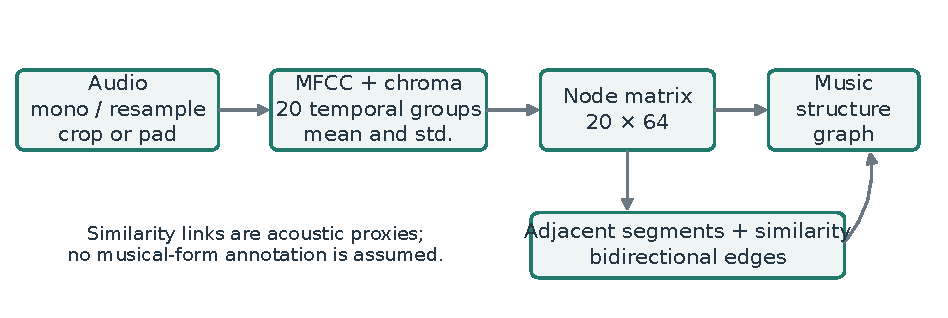
\includegraphics[width=0.92\linewidth]{fig2_graph_pipeline.pdf}
\caption{Audio graph construction. MFCC/chroma segment statistics form the nodes; temporal adjacency and acoustic similarity define bidirectional edges. Similarity is a proxy for recurrence, not ground-truth repetition or musical-form annotation.}
\label{fig:graph}
\end{figure*}

\section{Methodology}
\subsection{BERT baseline}
The caption encoder used is "distilbert-base-uncased," and At most 128 tokens per sequence, input sequences were cut short. Let Htext $\in$ R Lt$\times$dt refers to the token states, and t = Htext[0,:] is the first token. CLS-style representation. During Task 1 the following direct linear head was used.
\begin{equation}
\ell^{\mathrm{text}}=W_t t+b_t,\qquad
p^{\mathrm{text}}=\sigmoid(\ell^{\mathrm{text}}).
\label{eq:text}
\end{equation}
There was no intermediate MLP. Optimization of the encoder and classification head was done using Equation 2. Predictions and some sample captions, true tags, top-ranked tag probabilities, token sequences, and attention weights. For the last Transformer head, first-token attention was averaged across heads:
\begin{equation}
\bar a_j=\frac{1}{M}\sum_{m=1}^{M}a^{(\mathrm{last},m)}_{0j}.
\end{equation}
This is a diagnostic view of token attention, NOT a class-specific one! Causal explanation for a tag prediction [9]. Figure 3 presents

\begin{figure*}[t]
\centering
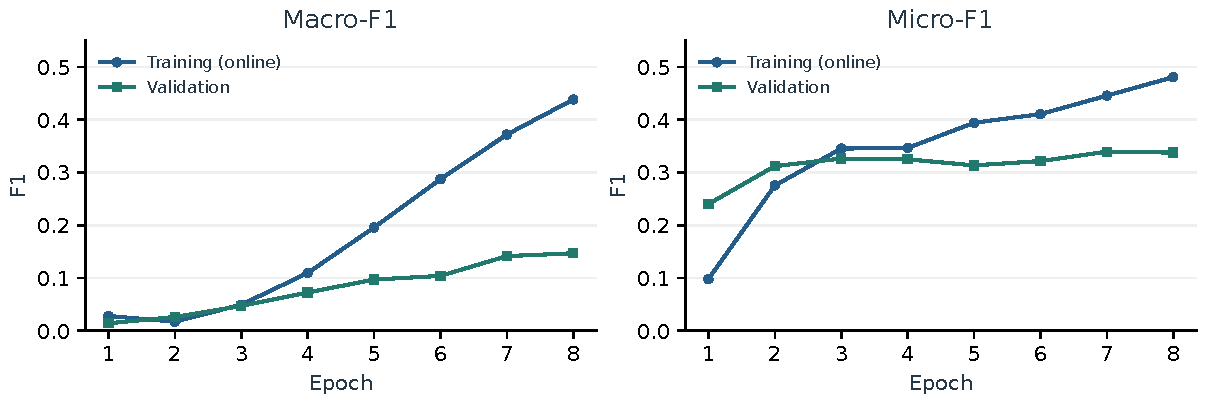
\includegraphics[width=0.92\linewidth]{fig3_bert_curves.pdf}
\caption{Task~1 Macro-/Micro-F1 across the eight training epochs, replotted from the saved CSV. Training values aggregate predictions collected during optimizer updates; validation values use evaluation mode after each epoch. These are not test-set learning curves.}
\label{fig:bertcurves}
\end{figure*}

\subsection{Music structure graph construction}
The 20 nodes were used in each clip graph, and the dimension of the nodes was 64. MFCC/chroma statistics. Sequential edges connected neighboring segments. Other similarity edges connect segments that are acoustically related---perhaps not contiguous. The connections were two-way, that is, messages could propagate in both directions. Each clip was treated as a separate unit, and There were no graph edges between training and test clips. This is a local continuity prior to this graph construction. with a content-based relation together. An acoustically similar may also be repeated instrumentation or texture, The procedure does not make it a repeated procedure. musical phrase. Adjacency edges combined with edge types. With no separately trained relation-specific mechanism and supplied to GraphSAGE. A graph also summarizes the global pooling. Instead of creating an explicit musical-form sequence.

\subsection{GraphSAGE encoder}
We implemented PyTorch Geometric SAGEConv (mean neighborhood aggregation). With initial features ( i 0) = xi , its conceptual update is
\begin{align}
m_i^{(l)}&=\operatorname{MEAN}_{j\in\mathcal{N}(i)}h_j^{(l)},\\
h_i^{(l+1)}&=\sigma\!\left(W^{(l)}\concat(h_i^{(l)},m_i^{(l)})\right).
\label{eq:sage}
\end{align}
In the conceptual expression, the affinely transformed features at the node and the neighbor are used, and the parameters of mean aggregation are shifted to the mean level by the SAGEConv. The parameters of mean aggregation are shifted to the mean level by the SAGEConv, and the affinely transformed features at the node and the neighbor are used. The saved encoder did normalization and Nonlinear activations around the graph updates. Its graph-level representation was
\begin{equation}
g=\frac{1}{|V|}\sum_{i\in V}h_i^{(L)}.
\label{eq:pool}
\end{equation}
The linear multi-label classifier converted g into logits. The implemented a standalone GraphSAGE encoder that did not contain Task 3 showed dropout/dropout present in shared task 3 feed-forward. head. This distinction is after the saved implementation: More than a generic description of the GraphSAGE design.

\subsection{Mel-spectrogram CNN baseline}
A 128-bin mel spectrogram was obtained for the acoustic baseline. Convolutional blocks incorporated batch normalization, ReLU, and. The classifiers used are pooling, adaptive global pooling, and the linear multi-label classifier. Spectrogram normalization was done per clip. Both CNN and standalone GraphSAGE were trained with the same prepared examples, vocabulary, 30-epoch budget, batch size, and 4 F1 F1 learning rate. They focused on different aspects of their input and how they were structured. Thus, the comparison tests these complete model pipelines. rather than just isolating connectivity of graphs.

\subsection{GNN--BERT fusion}
The graph readout provides the query and Keys and values are provided in the text sequence. Suppressing batch and head indices, which is a simplified description of
\begin{align}
Q&=gW_Q,\quad K=H_{\mathrm{text}}W_K,\quad V=H_{\mathrm{text}}W_V,\\
A&=\softmax\!\left(\frac{QK^\top}{\sqrt{d_k}}+M_{\mathrm{pad}}\right),\quad c=AV,
\label{eq:attention}\\
z&=\concat(g,c),\quad p=\sigmoid\!\left(f_{\mathrm{head}}(z)\right).
\label{eq:fusion}
\end{align}
Here, the Mpad does not include padding positions. The implementation implements a graph-to-text query projection, a multihead attention With an internal projection and an output projection. Thus the The attended text value is denoted by the shorthand CONCAT(g, AHtext). not raw tokens projected in space, but raw tokens projected in space. The feed-forward head Converts concatenated representation to label logits. Figure 4 illustrates the operation. The four Task 3 variants used t alone (BERT-only), g alone Only using a GNN, early concatenation (CONCAT(g,t)), or cross-attention (Equation 10). In this report, ``early concatenation'' 'means' is not to concatenate the encoder outputs before prediction. Raw audio sample concatenating and text tokens. All variants Incorporated and used the common feed-forward prediction design, including an An intermediate nonlinear layer and dropout. Task 3's BERT-only The direct linear Task 1 classifier and variant are different. as well as from it in the training budget. Implemented affect support. The model also contains valence/arousal outputs and supports.
\begin{equation}
\mathcal{L}=\mathcal{L}_{\mathrm{tags}}+\alpha\mathcal{L}_v+\beta\mathcal{L}_a,
\label{eq:multitask}
\end{equation}
where each auxiliary term is the mean squared error over finite, observed targets only. Alternatively, the mask of Lv is the same as the mask of La. The normed and normed versions of the difference between v and v\textasciicircum{}. 2 2 and $\Vert$a - a\textasciicircum{}$\Vert$ 2 2 When a target set is empty, its contribution is omitted. The configured coefficients of $\alpha$ = $\beta$ = 0.2. Evaluated objective. The Local MusicCaps subset did not have any DEAM valence/arousal annotations. Consequently, All reported Task 3 training runs optimized for tag loss only. The affect outputs were implemented but were not trained through Emotions are observed and/or assessed for emotion regression. Corresponding metrics were not stored as zero valued but instead as null. errors. Neither an affect-prediction benefit nor a multi-task approach was used. These results are indicative of supervision benefits.

\begin{figure*}[t]
\centering
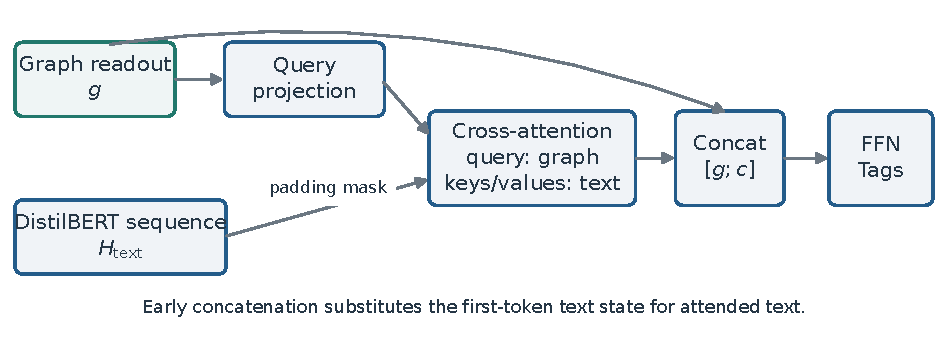
\includegraphics[width=0.92\linewidth]{fig4_fusion.pdf}
\caption{Task~3 cross-attention fusion. A graph-derived query attends to caption token states with padding masked. The attended text and original graph vector are concatenated before feed-forward classification.}
\label{fig:fusion}
\end{figure*}

\subsection{Contrastive dual encoder}
In Task 4, we trained an audio encoder (GraphSAGE) and a DistilBERT model. Separate 256-dimensional projections in a caption encoder. Both embeddings were L2 normalized:
\begin{equation}
u_i=\frac{P_g(g_i)}{\|P_g(g_i)\|_2},\qquad
v_i=\frac{P_t(t_i)}{\|P_t(t_i)\|_2}.
\end{equation}
The dot product is called the cosine similarity, si j = u. $\top$ i vj . For paired diagonal entries match examples and In-batch negatives are provided by the off-diagonal entries. With positive learnable temperature $\tau$, symmetric InfoNCE is
\begin{align}
\mathcal{L}_{A\rightarrow T}&=-\frac{1}{B}\sum_{i=1}^{B}
\log\frac{\exp(s_{ii}/\tau)}{\sum_{j=1}^{B}\exp(s_{ij}/\tau)},\\
\mathcal{L}_{T\rightarrow A}&=-\frac{1}{B}\sum_{i=1}^{B}
\log\frac{\exp(s_{ii}/\tau)}{\sum_{j=1}^{B}\exp(s_{ji}/\tau)},\\
\mathcal{L}_{\mathrm{NCE}}&=\tfrac12(\mathcal{L}_{A\rightarrow T}+\mathcal{L}_{T\rightarrow A}).
\label{eq:nce}
\end{align}
Both encoders were optimized. Figure 6 shows this independent retrieval architecture. A contrastive (CT) approach was used and then followed by No reported experiments involved tag fine-tuning.

\section{Experimental Setup}
\subsection{Training protocol}
The prepared split and random seed 42 were used for all experiments. The highest validation Macro-F1 was used to select classification checkpoints, and the maximum prediction threshold was set to 0.5. The The mean of six validation retrieval checkpoints was selected. In both directions recall values: R@1, R@5, and R@10. The Test retrieval was computed after the selection of epoch 19 as the selected retrieval checkpoint. Table 2 shows the prime settings. We have trained the four Task 3 variants for the same four epochs = 8, batch size = 8, pretrained = separate rates The parameters of text and new layers. Matching these settings Does not define a training schedule but does not assign meaning to parameter counts, initialization trajectories, or computational cost. Tasks 1 and 2 had separate longer training budgets. Results Within Task 3 are descriptive comparisons; across tasks are quantitative comparisons. Matched-budget fusion ablations are provided by experiment.

\begin{table*}[t]
\centering\small
\caption{Main experimental settings. A dash denotes a modality or setting that does not apply. The Task~3 affect coefficients were configured but inactive because emotion labels were unavailable.}
\label{tab:hyper}
\begin{tabular}{@{}lccccc@{}}
\toprule
Setting & Task 1 & Task 2: GraphSAGE & Task 2: CNN & Task 3: all variants & Task 4\\
\midrule
Epochs & 8 & 30 & 30 & 4 & 20\\
Batch size & 16 & 16 & 16 & 8 & 32\\
Text encoder learning rate & $2\!\times\!10^{-5}$ & --- & --- & $2\!\times\!10^{-5}$ & $2\!\times\!10^{-5}$\\
New-layer / audio learning rate & $2\!\times\!10^{-5}$ & $10^{-3}$ & $10^{-3}$ & $10^{-3}$ & $10^{-3}$\\
Maximum text tokens & 128 & --- & --- & 128 (text variants) & 128\\
Graph nodes / features & --- & 20 / 64 & --- & 20 / 64 (graph variants) & 20 / 64\\
Mel bins & --- & --- & 128 & --- & ---\\
Retrieval projection dimension & --- & --- & --- & --- & 256\\
Classification threshold & 0.5 & 0.5 & 0.5 & 0.5 & ---\\
Checkpoint criterion & Val. Macro-F1 & Val. Macro-F1 & Val. Macro-F1 & Val. Macro-F1 & Mean val. recall\\
Random seed & 42 & 42 & 42 & 42 & 42\\
\bottomrule
\end{tabular}
\end{table*}

\subsection{Evaluation metrics}
In case c: Compute true positives T Pc, false positives FPc, and False negative after thresholding FNc. Then
\begin{align}
F_{1,c}&=\frac{2TP_c}{2TP_c+FP_c+FN_c},\\
F_1^{\mathrm{macro}}&=\frac{1}{C}\sum_{c=1}^{C}F_{1,c},\\
F_1^{\mathrm{micro}}&=\frac{2\sum_cTP_c}{2\sum_cTP_c+\sum_cFP_c+\sum_cFN_c}.
\label{eq:f1}
\end{align}
If a label has an undefined value, then it is set to zero. Macro-F1 gives All labels are equal, while the Micro-F1 makes decisions. is more strongly affected by labels that have a lot of positives. Both are needed for the imbalanced vocabulary. Weighted BCE is also reported for Task 1; the saved loss is the The average loss from the evaluation script for mini-batches of data. Each of the 114 test queries is compared to In the other modality, all 114 candidates. A query has one designated matching item. If ri is its rank, then
\begin{equation}
R@K=\frac{1}{N}\sum_{i=1}^{N}\mathbb{1}[r_i\leq K],
\qquad K\in\{1,5,10\}.
\label{eq:recall}
\end{equation}
The metric is calculated individually for audio-to-caption and caption-to-audio retrieval. These recalls are valid for the exact pair ranking and should not be compared to classification numerically. F1 was taken to compare to the same task.

\section{Results}
The following classification numbers are for the test set that was not used to train the model. Unless explicitly stated as "validation," do not use. Values are rounded to Saved metrics to four decimals. No confidence intervals or Significance tests were calculated.

\subsection{Task 1: caption-only classification}
The direct DistilBERT classifier performed slightly better with a macro-F1 score of 0.1622. Micro-F1 of 0.3392, and weighted BCE loss of 0.6533 after Selection from 8 epochs based on validation. The learning As seen from Figure 3, validation Macro-F1 scores improved with the increase in training iterations, while the difference between training and validation scores increased. Because training predictions were collected online during updates, the plotted A gap is a descriptive diagnostic, not a precise match. evaluation-mode generalization estimate. The greater the micro-F1, the better the aggregate is. Better performance of frequent tags than the average tag. Based on the text of the captions, the retained system was supervised. Although metadata labels, macro-F1 will show that broad It continued to be hard to be recognized in the long tail. Five exported attention samples are diagnostic; they do Not be a quantitative explanation-faithfulness study.

\subsection{Task 2: Graph versus Convolutional Audio Modeling}
The two audio models with 30 epochs are compared in Table 3. GraphSAGE obtained a macro-/micro-F1 of 0.1006/0.2936, which improved over the results of the other methods. with 0.0873/0.2033 for the mel-CNN. The absolute improvements were 0.0133 and 0.0903, respectively. It's the greatest endorsement. The same was true for macro-F1. The result is a call for further structural investigation of audio. The current system of representations. Does not isolate. the contribution of recurrence edges: the systems differed in These include feature construction, normalization, architecture, and pooling. A nongraph (without similarity edges), a feature-matched nongraph attribute, or a wider CNN search would be needed to attribute In particular, the gain is used to graph connectivity.

\begin{table}[t]
\centering\small
\caption{Task~2 audio comparison under the same split and 30-epoch budget. Differences are absolute F1 values.}
\label{tab:audio}
\begin{tabular}{@{}lrrr@{}}
\toprule
Model & Best val. macro & Test macro & Test micro\\
\midrule
GraphSAGE & 0.1522 & \textbf{0.1006} & \textbf{0.2936}\\
Mel-CNN & 0.1175 & 0.0873 & 0.2033\\
Difference & --- & +0.0133 & +0.0903\\
\bottomrule
\end{tabular}
\end{table}

\subsection{Task 3: controlled fusion ablation}
The best validation and test results were obtained by early concatenation. Macro-F1 and the other equal budget variants (Table 4; Figure 5). Its test Macro-/Micro-F1 was 0.1770/0.3361. BERT-only reached 0.1096/0.2873, GNN-only reached 0.0375/0.2555, and Cross-attention reached 0.0685/0.2628. Combining graph and Initially the output of text representations was helpful for the purposes of concatenation. They found that in this experiment, they benefited as much from an unimodal variant to both variants and adding cross-attention to the unimodal. The contradiction between the Task 1 BERT Macro-F1 of 0.1622 and the Task 3 BERT-only Macro-F1 of 0.1096 does not exist. Task 1 used 8 epochs, 16 samples per batch, a direct linear classifier. Task 3 The \$4\textasciicircum{}\{th\}\$ epoch, \$8\$ batch size, a common non-linear prediction head, and a different learning rate for pretrained/new layers. The answer to the controlled-ablation question is addressed in the Task 3 result; and is not a repeat of task 1.

\begin{table}[t]
\centering\small
\caption{Task~3 ablation. All variants used four epochs and the common Task~3 prediction design. Emotion regression was not evaluated; no affect metrics are imputed.}
\label{tab:ablation}
\begin{tabular}{@{}lrrr@{}}
\toprule
Variant & Best val. macro & Test macro & Test micro\\
\midrule
Cross-attention & 0.0620 & 0.0685 & 0.2628\\
BERT-only & 0.1068 & 0.1096 & 0.2873\\
GNN-only & 0.0278 & 0.0375 & 0.2555\\
Early concat. & \textbf{0.1818} & \textbf{0.1770} & \textbf{0.3361}\\
\bottomrule
\end{tabular}
\end{table}

\begin{figure*}[t]
\centering
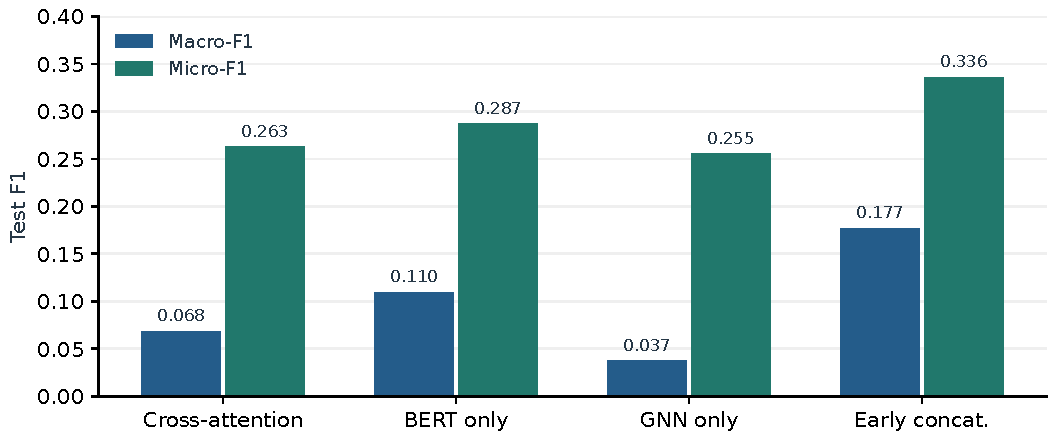
\includegraphics[width=0.85\linewidth]{fig5_ablation.pdf}
\caption{Task~3 test Macro-/Micro-F1 from the saved ablation table. Bars represent single-seed results; error bars are omitted because repeated-seed estimates were not available.}
\label{fig:ablation}
\end{figure*}

\subsection{Task 4: graph--caption retrieval}
The mean loss over the 20 epochs of the contrastive model runs was plotted. The six validation recalls are obtained from the list of epochs, and epoch 19 is chosen. It's held out. Results are given in Table 5. Audio-to-caption R@1/5/10 were 0.0614/0.2368/0.3772, while caption-to-audio values were 0.0789/0.2193/0.3860. The dual-encoder formulation used for these rankings is presented in Figure 6. There was a significant hike from first position to top ten. This pattern, coupled with performance exceeding the theoretical random-ranking reference, confers the support of non-trivial alignment. where K is the number of candidates for one candidate, this is an analytical reference, not an actual number of candidates. an additional trained baseline. However, both the forward and reverse matches were poor with R@1; thus, further precision matching was significantly achieved. More challenging than re-entering the pair in a larger candidate list.

\begin{table}[t]
\centering\small
\caption{Task~4 held-out exact-pair retrieval over 114 candidates per query, using the validation-selected epoch-19 model.}
\label{tab:retrieval}
\begin{tabular}{@{}lrrr@{}}
\toprule
Direction & R@1 & R@5 & R@10\\
\midrule
Audio graph $\rightarrow$ caption & 0.0614 & 0.2368 & 0.3772\\
Caption $\rightarrow$ audio graph & 0.0789 & 0.2193 & 0.3860\\
\bottomrule
\end{tabular}
\end{table}

\begin{figure*}[t]
\centering
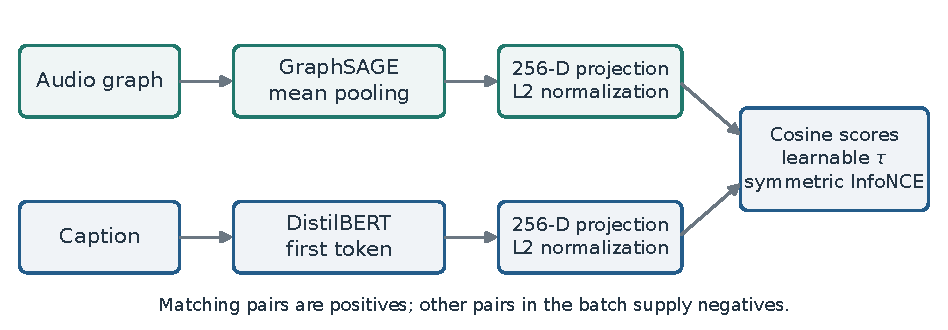
\includegraphics[width=0.92\linewidth]{fig6_contrastive.pdf}
\caption{Contrastive graph--caption encoder schematic. Separate 256-dimensional projections are L2-normalized and trained with symmetric InfoNCE. This is an architectural diagram, not an embedding visualization or a qualitative retrieval example.}
\label{fig:dual}
\end{figure*}

\subsection{Consolidated classification results}
The seven classifications are provided in one reference in Table 6. runs. The highest observed macro-F1 was for early concatenation. The best observed micro-F1 was for Task 1 DistilBERT. There was no single classifier that received both aggregate metrics for the separately budgeted tasks. The table preserves Do not assign the same task and epoch labels to all rows (as this would be equivalent to a fully single task). controlled architectural ranking.

\begin{table}[t]
\centering\small
\caption{Consolidated test classification results. Cross-task training budgets differ; boldface identifies numerical maxima, not statistical superiority. Retrieval is reported separately in Table~\ref{tab:retrieval}.}
\label{tab:all}
\begin{tabular}{@{}llrrr@{}}
\toprule
Task & Model & Epochs & Macro-F1 & Micro-F1\\
\midrule
1 & DistilBERT & 8 & 0.1622 & \textbf{0.3392}\\
2 & GraphSAGE & 30 & 0.1006 & 0.2936\\
2 & Mel-CNN & 30 & 0.0873 & 0.2033\\
3 & Cross-attention & 4 & 0.0685 & 0.2628\\
3 & BERT-only & 4 & 0.1096 & 0.2873\\
3 & GNN-only & 4 & 0.0375 & 0.2555\\
3 & Early concat. & 4 & \textbf{0.1770} & 0.3361\\
\bottomrule
\end{tabular}
\end{table}

\section{Discussion}
\subsection{Semantic text and structural audio}
Captions alone provided helpful context prediction for RQ1. and obtained a higher F1 compared to the standalone. audio models. Human captions can directly refer to semantics. This benefit is realistic because of its attributes that match up with metadata tags. The comparison is not illustrated in that text. Encoders have an intrinsic ability to derive more information from the original waveform: The caption is a supplement to the human-generated input. Without these descriptions, an audio-only deployment would not have this information. unless they had been made by another system, which was not within this, study. In RQ2, in the matched 30-epoch schedule, GraphSAGE outperformed the implemented mELCNN. Separated segments could be linked by relations to enable the aggregation of recurring acoustic patterns. However, mean/std. MFCC/chroma Here, statistics and spectrogram learning are two different features. biases. The current evidence is in favor of the graph pipeline as a not a causal statement about recurrence edges or It has an advantage over convolution that is shared across all.

\subsection{Why simple fusion was effective}
Early concatenation proved to be the best variant for RQ3. according to the four-epoch protocol. It reveals a potent pre-trained The caption representation is also directly sent to the prediction head, in addition to Providing acoustic graph information. Cross-attention must Also, be familiar with the caption tokens that will be used in response to: the graph query. The model was trained using just 532 training examples and 124 classes. If the labels are imbalanced, learning these interactions will need to be more observations or other optimization schedules. There are some further parameters and optimization complexity. The software for training and lack of supervision for fine-grained graph- The negative cross-attention result can be plausibly explained by token correspondences. They were not tested but were instead memorized. isolated. No parameter-matched attention ablation, training budget sweep, and large data comparison were run. The outcome, therefore, is only that the implemented This data set favored the early-concatenation model. size and schedule. A metric trade-off is also evident when comparing. This is because early concatenation outperforms the other two approaches in terms of Macro-F1 scores over the classification runs. For longer sequences, Task 1 DistilBERT had a higher Micro-F1, and its average tag recognition was comparable to that of suggest. training schedule. This should not be interpreted as a claim that adding Audio enhances all tags or all evaluation criteria.

\subsection{Long-tail prediction and diagnostic attention}
More frequent labels lead to more opportunities for true positives and more errors in micro-F1 pool counts. Macro-F1 weighs each Label equally, even with minimal training support. Their gap is consistent with difficulty recognizing underrepresented. After the rare label filtering and positive weighting, labels were not identified. The overall statistics do not determine which specific That's where tags fill in. A fixed thresholding can also be Labeling is not well calibrated for different prevalences of poor health. The actual saved 1st attention sample is shown in figure 7. It reports the average attention over the last layer (CLS-style attention). heads, saving the order and the weights of the saved token. The five 8 Test F1 Exported samples were chosen in the order in which they appeared in the test dataset instead of in natural order. Meteorologists should choose Project 2 rather than Project 1 because it is more likely to yield a documented success/failure sampling scheme. They are examples that can be inspected only and not representative evidence of the explanation quality. The top-ranked probabilities of tags in the sample exports are different from the full thresholded The sets of predictions for F1.

\begin{figure*}[t]
\centering
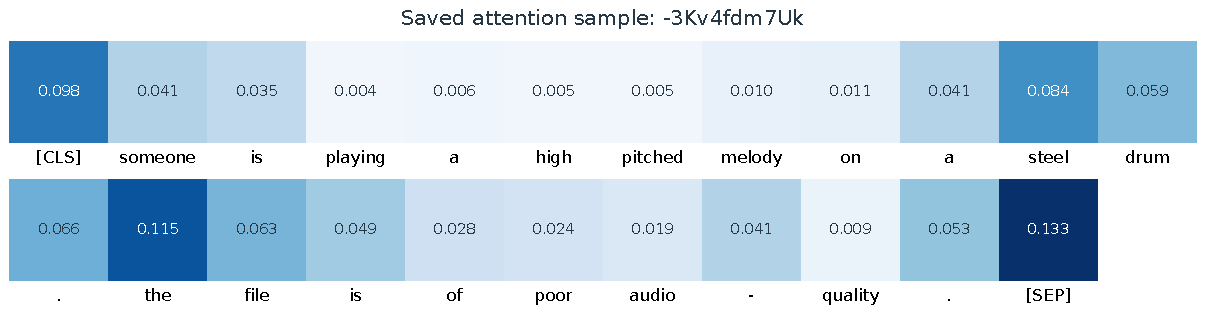
\includegraphics[width=0.92\linewidth]{fig7_attention.pdf}
\caption{One of five saved Task~1 attention samples, clip \pathcode{-3Kv4fdm7Uk}. Cell intensity and printed values show head-averaged final-layer attention from the first token. Tokens and values are replotted from the prediction JSON; no qualitative tag-attribution claim is inferred.}
\label{fig:attention}
\end{figure*}

\subsection{Retrieval scope}
In the case of RQ4, the bidirectional R@10 near 0.38 means that: Shared space stored data pertinent to an exact-pair ranking. in this test pool. Low R@1 indicates a significant part of the remaining ambiguity. Recall directions do not have to result in the same recall: One similar matrix is rank-ordered by rows, the other by columns. While the others have ands and columns. For exact-pair relevance, the level of relevance is high. Another caption can describe The same instrumentation, or texture, but is marked wrong because it is for a different clip. Conversely, good Retrieval does not have to be limited to these common acoustic features. Complete musical understanding demonstrated. No semantic relevance annotation, human evaluation, t-SNE analysis, or No retrieval case study is supplied (qualitative). To describe particular retrieved neighbors.

\section{Limitations and Future Work}
\subsection{Limitations}
The main constraint is size---there are 760 usable examples of Of which 532 were used for training, support 124 imbalanced labels. Part of the original vocabulary was filtered by frequency, and the corpus-level filtering determined the label universe. on the locally acquired subset. Results are thus not a measure of the coverage of all original tags or generalization to the full population of tags, MusicCaps population. One seed was used for all experiments. No mean/standard-deviation The task is to estimate the values of the parameters, their corresponding confidence intervals, or their significance. Tests were produced. A fixed value of 0.5 was used for classification. without per-label calibration. The decisions leave uncertainty. Discuss sensitivity to initialization, split composition, and the precision--recall operating point. Reproducible seeds also do Could not build a bitwise identity across versions of hardware and libraries. Very little was done in terms of architecture and hyperparameter tuning. This was the only major language encoder that was assessed; the audio graph was fixed in place and used edges built from features Four epochs were given to Task 3 for each variant. There were differences in the cross-task schedules and prediction heads. Consequently, none of The comparisons set the universal superiority of a model. family. Since no DEAM valence/arousal annotations were available, evaluated emotion predictions were not obtained with implemented affect heads. Retrieval of exact pairs (N=114) could be penalized. semantically valid alternatives and doesn't set any performance for a large search collection. IDs were disjointed, but Artist/recording-aware grouping and more general source contents. The saved split did not show leakage analysis. The captions can be used to provide explicit information about the tags of interest; this is inherent in the selected multimodal task, and it is easy to compare with purely acoustic understanding.

\subsection{Future work}
The successive evaluation steps involve repeated-seed runs, validation only per label threshold calibration, and reporting uncertainty. and per-tag behavior. More of the following data expansion could be used: If audio is available, a 5,521-pair MusicCaps release, Explore FMA and MagnaTagATune using clearly reasoned around label spaces. DEAM supervision would allow for actual The training and evaluation of the existing affect heads. These are Proposed extensions, not completed experiments. Representation studies might involve a comparison of pretrained audio encoders, GAT or graph transformer variants, learned edge construction, and beat-synchronous segmentation. It would be helpful if there was an edge ablation and a feature matched the nongraph baseline. Explain the contribution of the present graph. A larger or more carefully tuned attention model could then be used to determine if a student consistently understands and applies its instruction. The negative fusion result lasts for more than 4 epochs. To align, contrastive pre-training, classification fine-tuning, and hard-negative mining and retrieval with a larger size Pools are possible directions. Semantic relevance judgments would be used in conjunction with exact-pair recall. Artist-aware or recording-aware grouping should be used if there is metadata. permit it. None of the gains from these extensions are taken for granted in the current report.

\section{Reproducibility and Verification}
The project is structured as a Python package that can be installed. The modules are grouped into six core modules: data.py, audio.py, datasets.py, models.py, metrics.py, and training. py. Five entries The four experiments and data preparation are done in scripts: prepare\_data.py, train\_bert.py, train\_gnn.py, train\_fusion.py, and train\_contrastive. py. It is implemented by PyTorch, Transformers, and PyTorch Geometric. Librosa, scikit-learn, Matplotlib, pandas, and NumPy. Experiment outputs cover configurations in JSON and are saved. Vocabularies, CSV/JSON histories, validation-selected checkpoints, and held-out metrics. Graph and mel caches reduce repeated preprocessing. The Python and NumPy packages are provided as a part of shared utilities. and PyTorch, select CPU/GPU devices, and compute positive. Lift and transfer sets of tokens. configurable thresholds and learn rates; pretrained text parameters and configurable; Different rates may be used for new layers. Task 3 is needed to be invoked. Since its epoch 4 to reproduce the reported budget, its The default is different when using the command line. The package says that it supports Python 3.11 to 3.14; that range Is not an indication of testing of all interpreter versions. Practical compatibility work involved setting a writable Librosa/Numba cache location, choosing the Transformer attention to be paid to, and updating the version of the cache file to be compatible with the CLT. Settings that reveal attention tensors, dealing with DistilBERT Non-interactive Matplotlib rendering, reporting of regression targets when they don't exist, and not including "token\_type\_ids"---limit"-per-split allows for smokey runs; only full prepared-split runs were used for the reported results. Verification of source compilation, split integrity, real data, and analysis accuracy. The features being extracted, which are learned from the data, are related to the audio, graph, and mel tensor shapes as well as finite difference. values, and forward passes through GraphSAGE, the CNN, The DistilBERT, cross-attention, and contrastive dual encoder. The behavior of attention extraction and multi-task loss was evaluated. The end-to-end smoke tests and training on all prepared examples in each assigned split were followed. Passed all 6 unit tests. They include tag parsing, multi-hot encoding, split completeness/disjointness, multi-label F1, bidirectional retrieval, and more. retrieval-shape validation. These checks complement the uncertainty in the model and are not a substitute for model-level uncertainty. analysis. Measured figures were recreated from the saved outputs; architectural schematics illustrate the implementation. No new A training or retrieval experiment was used to produce a report. assets.

\section{Conclusion}
This project explored the semantics of captions, structural audio modelling, multimodal fusion, and contrastive alignment on a limited MusicCaps subset. DistilBERT gave a helpful semantic. The baseline model is the model implemented with the mel spectrogram CNN, which is improved by GraphSAGE with a matched training schedule of 30 epochs. Under The early concatenation feature is also a controlled four-epoch fusion budget. The early concatenation feature is also a controlled four epoch fusion budget. The best Macro-/Micro-F1 pair for the ablation variants was 0.1770/0.3361, which was achieved by the ablation variant. The Micro-F1 scores of the separate 8-epoch DistilBERT classifier (0.3392) highlighted its emphasis on the emphasis. the necessity of maintaining budget and head-design differences in comparing tasks. Cross-attention's weaker result indicates that there is more integration. Complexity was not a guarantee of improvement given the available supervision. Symmetric contrastive training also yielded useful graph--caption alignment, especially for the audio-to-caption alignment. and caption-to-audio R@10 of 0.3772 and 0.3860. The findings support simple fusion as a viable starting point in this context and stimulate future research on the structural audio features. The small sample size and label imbalance and single-seed evaluation are the issues that have to be addressed. Restrict the conclusions; valence/arousal regression continues. Implements functionality that was pending annotated data and experimental evaluation.

\FloatBarrier
\begin{thebibliography}{10}
\small
\bibitem{choi2016crnn}
K.~Choi, G.~Fazekas, M.~Sandler, and K.~Cho.
\newblock Convolutional Recurrent Neural Networks for Music Classification.
\newblock \emph{arXiv:1609.04243}, 2016.
\newblock \url{https://arxiv.org/abs/1609.04243}.

\bibitem{agostinelli2023musiclm}
A.~Agostinelli, T.~I.~Denk, Z.~Borsos, J.~Engel, M.~Verzetti, A.~Caillon, Q.~Huang,
A.~Jansen, A.~Roberts, M.~Tagliasacchi, M.~Sharifi, N.~Zeghidour, and C.~Frank.
\newblock MusicLM: Generating Music From Text.
\newblock \emph{arXiv:2301.11325}, 2023.
\newblock \url{https://arxiv.org/abs/2301.11325}.

\bibitem{devlin2019bert}
J.~Devlin, M.-W.~Chang, K.~Lee, and K.~Toutanova.
\newblock BERT: Pre-training of Deep Bidirectional Transformers for Language Understanding.
\newblock In \emph{NAACL-HLT}, pp.~4171--4186, 2019.
\newblock \href{https://aclanthology.org/N19-1423/}{doi:10.18653/v1/N19-1423}.

\bibitem{sanh2019distilbert}
V.~Sanh, L.~Debut, J.~Chaumond, and T.~Wolf.
\newblock DistilBERT, a distilled version of BERT: smaller, faster, cheaper and lighter.
\newblock \emph{arXiv:1910.01108}, 2019.
\newblock \url{https://arxiv.org/abs/1910.01108}.

\bibitem{hamilton2017graphsage}
W.~L.~Hamilton, R.~Ying, and J.~Leskovec.
\newblock Inductive Representation Learning on Large Graphs.
\newblock In \emph{Advances in Neural Information Processing Systems 30}, 2017.
\newblock \url{https://arxiv.org/abs/1706.02216}.

\bibitem{velickovic2018gat}
P.~Veli\v{c}kovi\'c, G.~Cucurull, A.~Casanova, A.~Romero, P.~Li\`o, and Y.~Bengio.
\newblock Graph Attention Networks.
\newblock In \emph{International Conference on Learning Representations}, 2018.
\newblock \url{https://arxiv.org/abs/1710.10903}.

\bibitem{elizalde2022clap}
B.~Elizalde, S.~Deshmukh, M.~Al~Ismail, and H.~Wang.
\newblock CLAP: Learning Audio Concepts From Natural Language Supervision.
\newblock \emph{arXiv:2206.04769}, 2022.
\newblock \url{https://arxiv.org/abs/2206.04769}.

\bibitem{oord2018cpc}
A.~van~den~Oord, Y.~Li, and O.~Vinyals.
\newblock Representation Learning with Contrastive Predictive Coding.
\newblock \emph{arXiv:1807.03748}, 2018.
\newblock \url{https://arxiv.org/abs/1807.03748}.

\bibitem{jain2019attention}
S.~Jain and B.~C.~Wallace.
\newblock Attention is not Explanation.
\newblock In \emph{NAACL-HLT}, pp.~3543--3556, 2019.
\newblock \href{https://aclanthology.org/N19-1357/}{doi:10.18653/v1/N19-1357}.

\bibitem{googlemusiccaps}
Google.
\newblock MusicCaps dataset.
\newblock Hugging Face Datasets; original dataset homepage on Kaggle. Accessed September 9, 2026.
\newblock \href{https://huggingface.co/datasets/google/MusicCaps}{Hugging Face dataset page};
\href{https://huggingface.co/datasets/google/MusicCaps/blob/main/musiccaps-public.csv}{public metadata CSV}.
\end{thebibliography}

\end{document}
